%!TEX TS-program = xelatex
%!TEX encoding = UTF-8 Unicode

\documentclass[12pt]{extarticle}
% extarticle is like article but can handle 8pt, 9pt, 10pt, 11pt, 12pt, 14pt, 17pt, and 20pt text

\def \ititle {Origins of Mind}
 
\def \isubtitle {Lecture 08}
 
\def \iauthor {Stephen A. Butterfill}
\def \iemail{s.butterfill@warwick.ac.uk}
\date{}

%for strikethrough
\usepackage[normalem]{ulem}

\input{$HOME/Documents/submissions/preamble_steve_handout}

%\bibpunct{}{}{,}{s}{}{,}  %use superscript TICS style bib
%remove hanging indent for TICS style bib
%TODO doesnt work
\setlength{\bibhang}{0em}
%\setlength{\bibsep}{0.5em}


%itemize bullet should be dash
\renewcommand{\labelitemi}{$-$}

\begin{document}

\raggedcolumns

\begin{multicols*}{3}

\setlength\footnotesep{1em}


\bibliographystyle{newapa} %apalike

%\maketitle
%\tableofcontents




%--------------- 
%--- start paste
\def \ititle {Logic I}
 
\def \isubtitle {Lecture 02}
 
\begin{center}
 
{\Large
 
\textbf{\ititle}: \isubtitle
 
}
 
 
 
\iemail %
 
\end{center}
 
Readings refer to sections of the course textbook, \emph{Language, Proof and Logic}.
 
 
 
\section{Recap: Validity, Counterexamples}
 
An argument is \emph{logically valid} just if there’s no possible situation in which the premises are true and the conclusion false
 
A \emph{counterexample} to an argument is a possible situation in which its premises are true and its conclusion false.
 
 
 
\section{Soundness}
 
An argument is \emph{sound} just if it is logically valid and its premises are true
 
Whether a sentence is true may change as the world changes.
 
The same applies to whether an argument is sound.
 
Whether an argument is logically valid not does change as the world changes.
 
 
 
\section{Identity}
 
\emph{Reading:} §2.2
 
Principle: If b=c then whatever is true of b is also true of c.
 
Principle: a=a is never false
 
\begin{center}
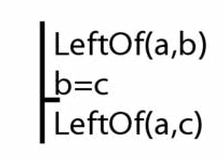
\includegraphics[scale=0.3]{img/arg_identity.png}
\end{center}
 
 
\section{Sentence Letters}
 
\begin{center}
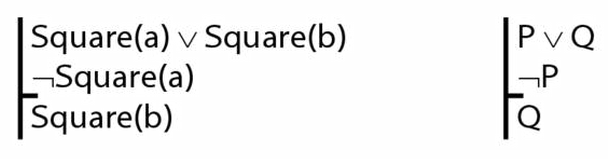
\includegraphics[scale=0.3]{img/sentence_letters.png}
\end{center}
 
 
\section{Truth Tables}
 
\emph{Reading:} §3.1, §3.2, §3.3
 
Rough guide:
 
`$\land{}$' means and
 
`$\lor{}$' means or
 
`$\lnot{}$' means not
 
\begin{center}
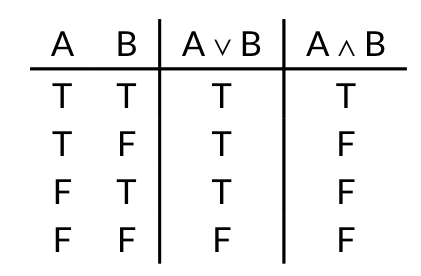
\includegraphics[scale=0.3]{img/truth_table_or_and.png}
\end{center}
\begin{center}
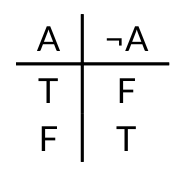
\includegraphics[scale=0.3]{img/truth_table_not.png}
\end{center}
 
 
\section{Complex Truth Tables}
 
\begin{center}
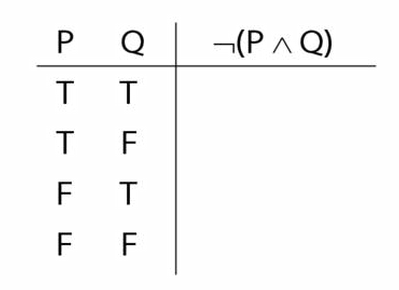
\includegraphics[scale=0.3]{img/unit_60_tt.png}
\end{center}
 
 
\section{Contradictions, Logical Truths and Logical Possibilities}
 
\emph{Reading:} §2.2
 
A \emph{contradiction} is a sentence that is false in all possible situations.
 
A \emph{logical truth} is a sentence that is true in all possible situations.
 
A \emph{logical possibility} is a sentence that is true in one or more possible situations.
 

%--- end paste
%--------------- 
 


\end{multicols*}

\end{document}